\documentclass{beamer}
\usetheme{Madrid} 
\usecolortheme{dolphin}

\makeatletter
\setbeamertemplate{headline}{%
  \begin{beamercolorbox}[wd=\paperwidth,ht=2.8ex,dp=1.2ex]{section in head/foot}%
    \hfill\insertsectionnavigationhorizontal{0.96\paperwidth}{}{}\hfill%
  \end{beamercolorbox}}
\setbeamertemplate{section in head/foot}{\hfill\insertsectionhead\hfill}
\setbeamertemplate{section in head/foot shaded}{\color{fg!50!bg}\usebeamertemplate{section in head/foot}}
\makeatother
\setbeamerfont{subsection in toc}{size=\footnotesize}

\setbeamertemplate{bibliography item}{\insertbiblabel}
\setbeamerfont{bibliography item}{size=\scriptsize}
\setbeamerfont{bibliography entry author}{size=\scriptsize}
\setbeamerfont{bibliography entry title}{size=\scriptsize}
\setbeamerfont{bibliography entry location}{size=\scriptsize}
\setbeamerfont{bibliography entry note}{size=\scriptsize}
\setbeamertemplate{frametitle continuation}{}

%% packages
\usepackage{amsmath}
\usepackage{amssymb}
\usepackage{bm}
\usepackage{booktabs}
\usepackage{tikz}
\usetikzlibrary{positioning,arrows.meta,calc}
\usepackage{textcomp}
\usepackage{appendixnumberbeamer}

\usepackage[style=ieee,backend=biber]{biblatex}
\addbibresource{references.bib}
\renewcommand{\footnotesize}{\scriptsize}

% macros.tex
% All custom commands live here.
% Loaded from main.tex with % macros.tex
% All custom commands live here.
% Loaded from main.tex with % macros.tex
% All custom commands live here.
% Loaded from main.tex with \input{macros}, after \input{packages}.
% (Requires the packages loaded in packages.tex: bbm, mathrsfs.)
 
% --- Operators and named quantities ---
\newcommand{\TN}{\mathsf{TN}}
\newcommand{\var}{\mathbb{V}\mathrm{ar}}   % variance
\newcommand{\cov}{\mathbb{C}\mathrm{ov}}   % covariance
\newcommand{\corr}{\mathbb{C}\mathrm{orr}} % correlation
\DeclareMathOperator*{\argmin}{argmin}
\DeclareMathOperator{\tr}{tr}
 
% --- Distribution / convergence relations ---
\newcommand{\simapprox}{\stackrel{\mathrm{approx}}{\sim}}
\newcommand{\simiid}{\stackrel{\mathrm{iid}}{\sim}}
\newcommand{\simiidt}{\sim_\mathrm{iid}}
\newcommand{\cas}{\stackrel{\mathrm{a.s.}}{\longrightarrow}} % converges almost surely
\newcommand{\cd}{\stackrel{\mathrm{d}}{\longrightarrow}}     % converges in distribution
\newcommand{\cp}{\stackrel{\mathbb{P}}{\longrightarrow}}     % converges in probability
 
% --- Font shorthands ---
\newcommand{\bb}[1]{\mathbb{#1}}       % blackboard bold
\newcommand{\m}[1]{\mathbf{#1}}        % upright bold (matrices)
\newcommand{\vv}[1]{\boldsymbol{#1}}   % bold italic (vectors)   [was \v: caron accent]
\newcommand{\mc}[1]{\mathcal{#1}}      % calligraphic            [was \c: cedilla accent]
\newcommand{\s}[1]{\mathscr{#1}}       % script
 
% --- Upright constants and differentials ---
\newcommand{\di}{\mathrm{d}}           % differential d
\newcommand{\e}{\mathrm{e}}            % Euler's number
\newcommand{\iu}{\mathrm{i}\,}         % imaginary unit          [was \i: dotless i]
\newcommand{\I}{\mathbbm{1}}           % indicator function
\newcommand{\gvn}{\,|\,}               % "given" bar for conditionals
 , after % packages.tex
% All \usepackage lines live here.
% Loaded from main.tex with \input{packages}, before \input{macros}.
\usepackage[a4paper, total={7in, 10in}]{geometry} % Set page and margins

% --- Maths ---
\usepackage{amsmath}     % core maths environments (align, etc.)
\usepackage{amssymb}     % extra symbols (\mathbb, etc.)
\usepackage{bm}          % bold maths symbols (\bm)
\usepackage{bbm}         % \mathbbm{1} for the indicator function
\usepackage{mathrsfs}    % \mathscr script font

% --- Add other thesis packages below as you need them, for example: ---
\usepackage{graphicx}          % figures
\usepackage{booktabs}          % nicer tables
\usepackage{physics}
\usepackage[dvipsnames]{xcolor} % coloured text
\usepackage{listings}

% Load hyperref LAST (after almost everything else):
\usepackage{hyperref}
\usepackage[acronym]{glossaries-extra}
.
% (Requires the packages loaded in packages.tex: bbm, mathrsfs.)
 
% --- Operators and named quantities ---
\newcommand{\TN}{\mathsf{TN}}
\newcommand{\var}{\mathbb{V}\mathrm{ar}}   % variance
\newcommand{\cov}{\mathbb{C}\mathrm{ov}}   % covariance
\newcommand{\corr}{\mathbb{C}\mathrm{orr}} % correlation
\DeclareMathOperator*{\argmin}{argmin}
\DeclareMathOperator{\tr}{tr}
 
% --- Distribution / convergence relations ---
\newcommand{\simapprox}{\stackrel{\mathrm{approx}}{\sim}}
\newcommand{\simiid}{\stackrel{\mathrm{iid}}{\sim}}
\newcommand{\simiidt}{\sim_\mathrm{iid}}
\newcommand{\cas}{\stackrel{\mathrm{a.s.}}{\longrightarrow}} % converges almost surely
\newcommand{\cd}{\stackrel{\mathrm{d}}{\longrightarrow}}     % converges in distribution
\newcommand{\cp}{\stackrel{\mathbb{P}}{\longrightarrow}}     % converges in probability
 
% --- Font shorthands ---
\newcommand{\bb}[1]{\mathbb{#1}}       % blackboard bold
\newcommand{\m}[1]{\mathbf{#1}}        % upright bold (matrices)
\newcommand{\vv}[1]{\boldsymbol{#1}}   % bold italic (vectors)   [was \v: caron accent]
\newcommand{\mc}[1]{\mathcal{#1}}      % calligraphic            [was \c: cedilla accent]
\newcommand{\s}[1]{\mathscr{#1}}       % script
 
% --- Upright constants and differentials ---
\newcommand{\di}{\mathrm{d}}           % differential d
\newcommand{\e}{\mathrm{e}}            % Euler's number
\newcommand{\iu}{\mathrm{i}\,}         % imaginary unit          [was \i: dotless i]
\newcommand{\I}{\mathbbm{1}}           % indicator function
\newcommand{\gvn}{\,|\,}               % "given" bar for conditionals
 , after % packages.tex
% All \usepackage lines live here.
% Loaded from main.tex with % packages.tex
% All \usepackage lines live here.
% Loaded from main.tex with \input{packages}, before \input{macros}.
\usepackage[a4paper, total={7in, 10in}]{geometry} % Set page and margins

% --- Maths ---
\usepackage{amsmath}     % core maths environments (align, etc.)
\usepackage{amssymb}     % extra symbols (\mathbb, etc.)
\usepackage{bm}          % bold maths symbols (\bm)
\usepackage{bbm}         % \mathbbm{1} for the indicator function
\usepackage{mathrsfs}    % \mathscr script font

% --- Add other thesis packages below as you need them, for example: ---
\usepackage{graphicx}          % figures
\usepackage{booktabs}          % nicer tables
\usepackage{physics}
\usepackage[dvipsnames]{xcolor} % coloured text
\usepackage{listings}

% Load hyperref LAST (after almost everything else):
\usepackage{hyperref}
\usepackage[acronym]{glossaries-extra}
, before % macros.tex
% All custom commands live here.
% Loaded from main.tex with \input{macros}, after \input{packages}.
% (Requires the packages loaded in packages.tex: bbm, mathrsfs.)
 
% --- Operators and named quantities ---
\newcommand{\TN}{\mathsf{TN}}
\newcommand{\var}{\mathbb{V}\mathrm{ar}}   % variance
\newcommand{\cov}{\mathbb{C}\mathrm{ov}}   % covariance
\newcommand{\corr}{\mathbb{C}\mathrm{orr}} % correlation
\DeclareMathOperator*{\argmin}{argmin}
\DeclareMathOperator{\tr}{tr}
 
% --- Distribution / convergence relations ---
\newcommand{\simapprox}{\stackrel{\mathrm{approx}}{\sim}}
\newcommand{\simiid}{\stackrel{\mathrm{iid}}{\sim}}
\newcommand{\simiidt}{\sim_\mathrm{iid}}
\newcommand{\cas}{\stackrel{\mathrm{a.s.}}{\longrightarrow}} % converges almost surely
\newcommand{\cd}{\stackrel{\mathrm{d}}{\longrightarrow}}     % converges in distribution
\newcommand{\cp}{\stackrel{\mathbb{P}}{\longrightarrow}}     % converges in probability
 
% --- Font shorthands ---
\newcommand{\bb}[1]{\mathbb{#1}}       % blackboard bold
\newcommand{\m}[1]{\mathbf{#1}}        % upright bold (matrices)
\newcommand{\vv}[1]{\boldsymbol{#1}}   % bold italic (vectors)   [was \v: caron accent]
\newcommand{\mc}[1]{\mathcal{#1}}      % calligraphic            [was \c: cedilla accent]
\newcommand{\s}[1]{\mathscr{#1}}       % script
 
% --- Upright constants and differentials ---
\newcommand{\di}{\mathrm{d}}           % differential d
\newcommand{\e}{\mathrm{e}}            % Euler's number
\newcommand{\iu}{\mathrm{i}\,}         % imaginary unit          [was \i: dotless i]
\newcommand{\I}{\mathbbm{1}}           % indicator function
\newcommand{\gvn}{\,|\,}               % "given" bar for conditionals
 .
\usepackage[a4paper, total={7in, 10in}]{geometry} % Set page and margins

% --- Maths ---
\usepackage{amsmath}     % core maths environments (align, etc.)
\usepackage{amssymb}     % extra symbols (\mathbb, etc.)
\usepackage{bm}          % bold maths symbols (\bm)
\usepackage{bbm}         % \mathbbm{1} for the indicator function
\usepackage{mathrsfs}    % \mathscr script font

% --- Add other thesis packages below as you need them, for example: ---
\usepackage{graphicx}          % figures
\usepackage{booktabs}          % nicer tables
\usepackage{physics}
\usepackage[dvipsnames]{xcolor} % coloured text
\usepackage{listings}

% Load hyperref LAST (after almost everything else):
\usepackage{hyperref}
\usepackage[acronym]{glossaries-extra}
.
% (Requires the packages loaded in packages.tex: bbm, mathrsfs.)
 
% --- Operators and named quantities ---
\newcommand{\TN}{\mathsf{TN}}
\newcommand{\var}{\mathbb{V}\mathrm{ar}}   % variance
\newcommand{\cov}{\mathbb{C}\mathrm{ov}}   % covariance
\newcommand{\corr}{\mathbb{C}\mathrm{orr}} % correlation
\DeclareMathOperator*{\argmin}{argmin}
\DeclareMathOperator{\tr}{tr}
 
% --- Distribution / convergence relations ---
\newcommand{\simapprox}{\stackrel{\mathrm{approx}}{\sim}}
\newcommand{\simiid}{\stackrel{\mathrm{iid}}{\sim}}
\newcommand{\simiidt}{\sim_\mathrm{iid}}
\newcommand{\cas}{\stackrel{\mathrm{a.s.}}{\longrightarrow}} % converges almost surely
\newcommand{\cd}{\stackrel{\mathrm{d}}{\longrightarrow}}     % converges in distribution
\newcommand{\cp}{\stackrel{\mathbb{P}}{\longrightarrow}}     % converges in probability
 
% --- Font shorthands ---
\newcommand{\bb}[1]{\mathbb{#1}}       % blackboard bold
\newcommand{\m}[1]{\mathbf{#1}}        % upright bold (matrices)
\newcommand{\vv}[1]{\boldsymbol{#1}}   % bold italic (vectors)   [was \v: caron accent]
\newcommand{\mc}[1]{\mathcal{#1}}      % calligraphic            [was \c: cedilla accent]
\newcommand{\s}[1]{\mathscr{#1}}       % script
 
% --- Upright constants and differentials ---
\newcommand{\di}{\mathrm{d}}           % differential d
\newcommand{\e}{\mathrm{e}}            % Euler's number
\newcommand{\iu}{\mathrm{i}\,}         % imaginary unit          [was \i: dotless i]
\newcommand{\I}{\mathbbm{1}}           % indicator function
\newcommand{\gvn}{\,|\,}               % "given" bar for conditionals
 
\graphicspath{{figs/}}

\setbeamertemplate{navigation symbols}{} 

\title[Target Detection in K-distributed Clutter]{Practical Radar Target Detection in K-distributed Clutter}
\author[]{Tian Huang}
\institute[]{Supervisor: Prof. Elias Aboutanios}
\date[]{\scriptsize November 9, 2026}

\begin{document}

{
\setbeamertemplate{headline}{}   % no header for these frames only
%% ----- Title ------ %%
\begin{frame}
  \titlepage
\end{frame}

%% ----- Outline ------ %%
\begin{frame}{Outline}
  \begin{columns}[T]
    \begin{column}{0.48\textwidth}
      \tableofcontents[sections={1-3}]
    \end{column}
    \begin{column}{0.48\textwidth}
      \tableofcontents[sections={4-6}]
    \end{column}
  \end{columns}
\end{frame}
}

%% ----- Section 1: Background ------ %%
\section{Background and Motivation}

%% 1.1 Radar Target Detection and its Applications
\subsection{Radar Target Detection}
\begin{frame}{Radar Target Detection}
    \begin{columns}[c]
        \begin{column}{0.55\textwidth}
            \begin{itemize}
                \item \textbf{Target detection:} deciding, for the cell under test (CUT), whether a target is present or not
                \item \textbf{Applications:} maritime surveillance, search and rescue, air traffic control
                \item The radar also receives unwanted signals: 
                \begin{itemize}
                    \item \textbf{Noise:} random thermal noise from the receiver electronics
                    \item \textbf{Clutter:} unwanted echoes from the environment, e.g. the sea surface
                \end{itemize}
            \end{itemize}
        \end{column}
        \begin{column}{0.42\textwidth}
            \centering
            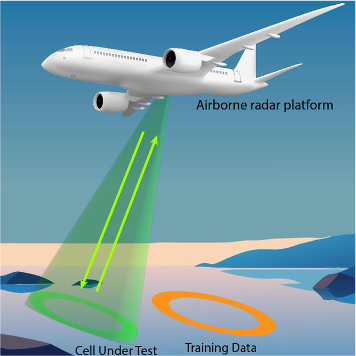
\includegraphics[width=\textwidth]{figs/radar_img.png}\\
            % {\tiny Image: [source]}
        \end{column}
    \end{columns}
    \begin{itemize}
        \item At sea, clutter can often be stronger than a small or slow target.
    \end{itemize}        
\end{frame}

%% 1.2 Real Clutter vs the Gaussian Assumption
\subsection{Real Clutter vs the Gaussian Assumption}
\begin{frame}{Real Clutter vs the Gaussian Assumption}
    \small
    \begin{columns}[T]
        \begin{column}{0.27\textwidth}
            \centering
            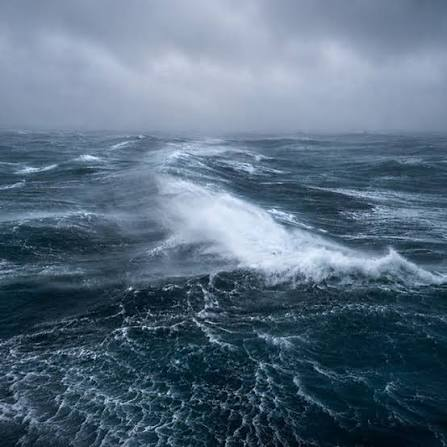
\includegraphics[width=\textwidth, height=2cm]{figs/breaking_waves.jpg}\\[2pt]
            \raggedright
            \textbf{Spiky}: breaking waves give bright \emph{sea spikes}
        \end{column}
        \begin{column}{0.27\textwidth}
            \centering
            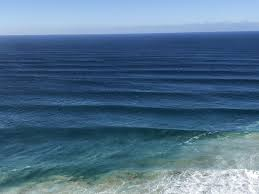
\includegraphics[width=\textwidth, height=2cm]{figs/swell_group.jpg}\\[2pt]
            \raggedright
            \textbf{Heterogeneous}: swell makes the echo power change cell to cell
        \end{column}
        \begin{column}{0.42\textwidth}
            \centering
            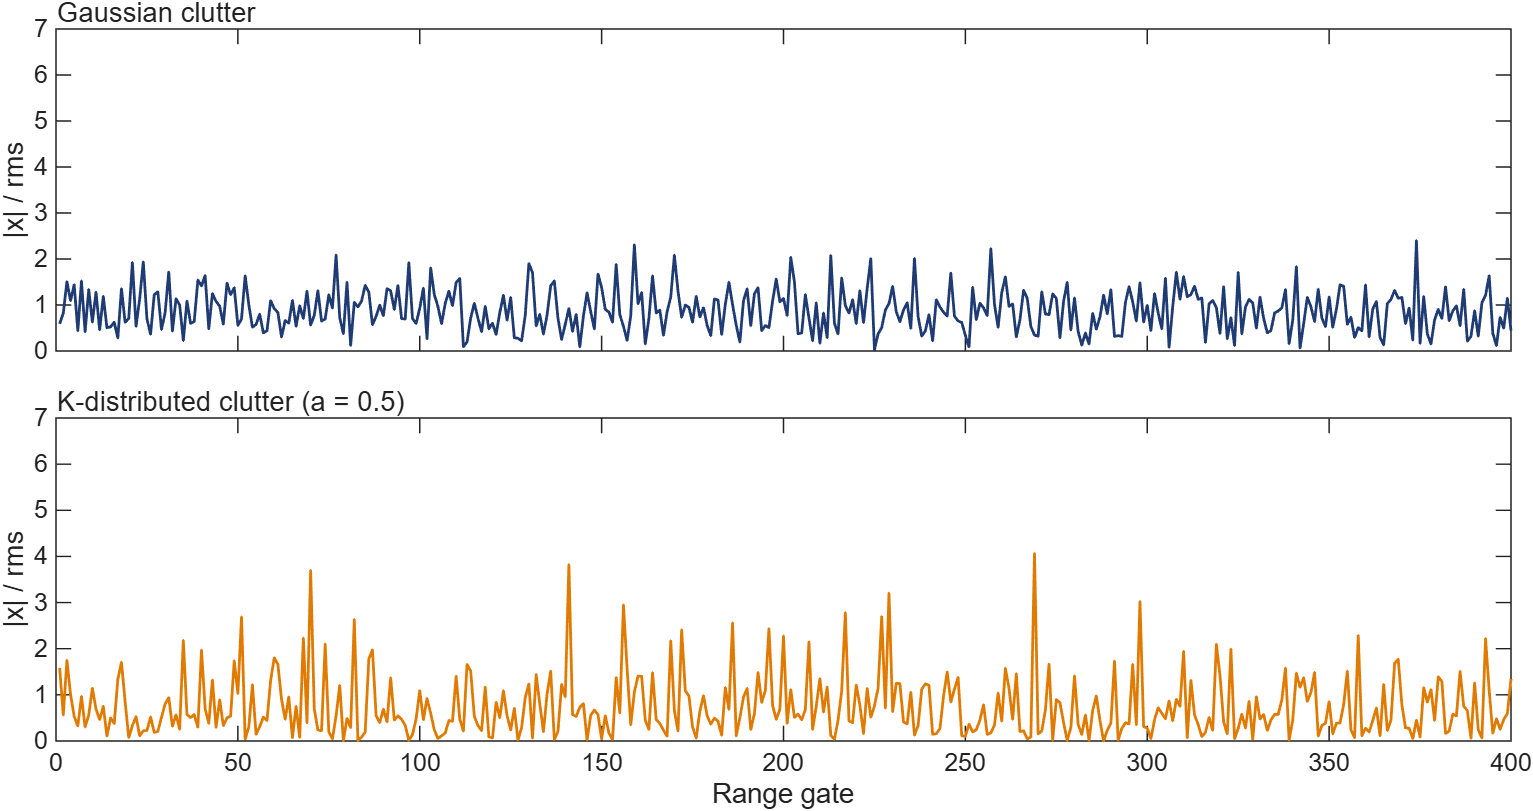
\includegraphics[width=\textwidth]{spiky.png}\\
            {\scriptsize Same average power: Gaussian vs K}
        \end{column}
    \end{columns}
    \vspace{3mm}
    \begin{itemize}
        \item So we model it as \textbf{K-distributed}, not Gaussian and homogeneous
        \item Standard detectors designed for Gaussian clutter $\rightarrow$ \textbf{false alarms} or \textbf{missed} small targets
    \end{itemize}
    \vspace{1mm}
    \begin{block}{The problem}
        How do we effectively detect a weak target in spiky, changing K-distributed clutter?
    \end{block}
\end{frame}

%% ----- Section 2: Detection Theory ----- %%
\section{Detection Theory}

%% 2.1 Radar Signal Model
\subsection{Radar Signal Model}
\begin{frame}{Radar Signal Model}
    \small
    \begin{columns}[c]
        \begin{column}{0.22\textwidth}
            \centering
            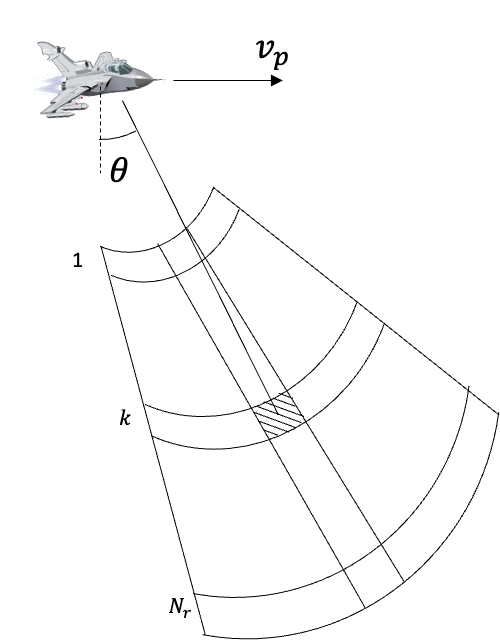
\includegraphics[height=3.1cm]{airborne_radar_signal_model.png}
        \end{column}
        \begin{column}{0.76\textwidth}
            \begin{itemize}
                \item Side-looking array: $N$ elements, spacing $d$, speed $v_p$
                \item Transmit one beam; receive on $N$ channels, over $M$ pulses 
                \item Each cell receives: $N\times M$ samples stacked into $\mathbf{x}\in\mathbb{C}^{L}$, $L = NM$
            \end{itemize}
        \end{column}
    \end{columns}
    \vspace{4mm}
    \begin{block}{Received vector in one range gate}
        \[ \mathbf{x} = \underbrace{\alpha\,\mathbf{s}}_{\text{target}} + \underbrace{\mathbf{c}}_{\text{clutter}} + \underbrace{\mathbf{n}}_{\text{noise}},
           \qquad \mathbf{s}(f_s,f_d) = \mathbf{s}_\text{temp}(f_d)\otimes\mathbf{s}_\text{sp}(f_s) \]
        \vspace{-3mm}
        \footnotesize
        \begin{itemize}
            \item Across elements, phase $\rightarrow$ \textbf{angle}: $f_s = d\sin\theta/\lambda$
            \item Across pulses, phase $\rightarrow$ \textbf{velocity}: $f_d = 2vT_r/\lambda$
        \end{itemize}
    \end{block}
\end{frame}

%% 2.2 Clutter and Noise Models
\subsection{Clutter and Noise Models}
\begin{frame}{Clutter and Noise Models}
    \small
    \textbf{Clutter}:$\;\mathbf{c} = \sqrt{\tau}\,\mathbf{q}$ (Compound-Gaussian model \cite{Gini1998})
    \vspace{1mm}
    \begin{columns}[T]
        \begin{column}{0.5\textwidth}
            \begin{itemize}
                \item \textbf{Speckle} $\mathbf{q}\sim\mathcal{CN}(\mathbf{0},\mathbf{G})$
                \item \textbf{Texture} $\tau\sim\Gamma(a, b)$
            \end{itemize}
        \end{column}
        \begin{column}{0.48\textwidth}
            \textbf{At sea}
            \begin{itemize}
                \item \textbf{Spiky}: random $\tau$ $\Rightarrow$ heavy-tailed amplitude
                \item \textbf{Heterogeneous}: $\tau_k$ differs cell to cell
            \end{itemize}
        \end{column}
    \end{columns}
    \vspace{8mm}
    \textbf{Noise:} $\mathbf{n}\sim\mathcal{CN}(\mathbf{0},\sigma^2\mathbf{I})$: white Gaussian receiver noise
    \begin{block}{Received vector in the CUT}
        \[ \mathbf{x}\mid\tau \sim \mathcal{CN}\big(\alpha\,\mathbf{s},\, \mathbf{R}\big), \qquad
           \mathbf{R} = \tau\mathbf{G} + \sigma^2\mathbf{I}\ \text{(clutter + noise covariance)} \]
        In practice, $\tau$ and $\m G$ are \textbf{unknown}, and as such, so is $\m R$.
    \end{block}
\end{frame}

%% 2.3 Hypothesis Testing and CFAR
\subsection{Hypothesis Testing}
\begin{frame}{Hypothesis Testing and CFAR}
    \small
    For each cell under test, decide between
    \[ H_0:\ \mathbf{x} = \mathbf{c} + \mathbf{n} \qquad\text{vs}\qquad
       H_1:\ \mathbf{x} = \alpha\,\mathbf{s} + \mathbf{c} + \mathbf{n} \]
    \vspace{-3mm}
    \begin{columns}[T]
        \begin{column}{0.5\textwidth}
            \textbf{Test statistic}: one number $y = T(\mathbf{x})$ that measures how target-like the cell is
            \begin{itemize}
                \item Decide $H_0$ (no target) if $y < \gamma$
                \item Decide $H_1$ (target) if $y \geq \gamma$
                \item False alarm $P_{fa} = P(y > \gamma \mid H_0)$
                \item Detection $P_d = P(y > \gamma \mid H_1)$
            \end{itemize}
        \end{column}
        \begin{column}{0.48\textwidth}
            \textbf{Neyman--Pearson} \cite{Neyman1933}: for a fixed $P_{fa}$, the highest $P_d$ comes from the \textbf{likelihood ratio}
            \[y = \frac{f_{\vb x}(\mathbf{x}\mid H_1)}{f_{\vb x}(\mathbf{x}\mid H_0)} \;\underset{H_0}{\overset{H_1}{\gtrless}}\; \gamma \]
            \vspace{-2mm}
            \begin{itemize}
                \item Choose $P_{fa}$ to be a maximum probability of false alarm that we can torelate, to set $\gamma$.
            \end{itemize}
        \end{column}
    \end{columns}
    \begin{block}{CFAR: constant false alarm rate}
        A usable detector must hold $P_{fa}$ fixed even though interference power is unknown and varies across the scene
    \end{block}
\end{frame}

%% ----- Section 3: Current Detectors ----- %%
\section{Current Detectors}

%% 3.1 Gaussian Adaptive Detectors
\subsection{Gaussian Adaptive Detectors}
\begin{frame}{Gaussian Adaptive Detectors}
    \small
    Applies likelihood ratio assuming \textbf{Gaussian} and \textbf{homogeneous} clutter
    \begin{center}
    \begin{tikzpicture}[box/.style={draw, rounded corners, fill=blue!10, align=center, font=\footnotesize, minimum height=0.9cm, text width=3.1cm, inner sep=3pt},
                        >=stealth, thick]
        \node[box] (a) at (0,0)    {\textbf{1. Assume}\\ every cell $\sim\mathcal{CN}(\mathbf{0},\mathbf{R})$, \textbf{same} $\mathbf{R}$};
        \node[box] (b) at (3.75,0) {\textbf{2. Likelihood ratio}\\ best test if $\mathbf{R}$ known};
        \node[box, fill=orange!25] (c) at (7.5,0) {\textbf{3. $\mathbf{R}$ unknown}\\ estimate from \textbf{training data}};
        \draw[->] (a) -- (b); \draw[->] (b) -- (c);
    \end{tikzpicture}
    \end{center}
    \vspace{-2mm}
    \[ \text{AMF \cite{Chen1991}:}\quad y_\text{AMF} = \frac{|\mathbf{s}^H\hat{\mathbf{R}}^{-1}\mathbf{x}|^2}{\mathbf{s}^H\hat{\mathbf{R}}^{-1}\mathbf{s}} \;\gtrless\; \gamma,
       \quad \hat{\mathbf{R}} = \text{sample covariance matrix} \]
    \vspace{-2mm}
    \begin{itemize}
        \item How well $\mathbf{x}$ matches the target signature $\mathbf{s}$, with the clutter suppressed
        \item Training cells must be \textbf{homogeneous}: i.i.d.\ with the CUT, \textbf{same} $\mathbf{R}$
        \item Others, e.g.\ NAMF \cite{Kraut1999}, GLRT \cite{Kelly1986}: similar and all CFAR in Gaussian clutter
    \end{itemize}
    \begin{alertblock}{In practice}
        The statistic and threshold $\gamma$ are set \textbf{assuming Gaussian, homogeneous clutter}. At sea the texture breaks both: detection drops and CFAR is lost \cite{Gini1998, Rosenberg2017}.
    \end{alertblock}
\end{frame}

%% 3.2 Optimum K-distributed Detector (OKD)
\subsection{Optimum K-distributed Detector}
\begin{frame}{Optimum K-distributed Detector (OKD) \cite{Gini1998}}
    \small
    Applies the same likelihood ratio test, but assuming \textbf{K-distributed} clutter
    \begin{block}{OKD test statistic}
        \[ y_\text{OKD} = \frac{p(\mathbf{x}\mid H_1)}{p(\mathbf{x}\mid H_0)} = \frac{h(q_1)}{h(q_0)} \;\underset{H_0}{\overset{H_1}{\gtrless}}\; \gamma,
           \qquad h(q) = \int_0^\infty \tau^{-L} e^{-q/\tau} f_\tau(\tau)\,d\tau \]
        \vspace{-1mm}
        \[ q_0(\vb x) = \mathbf{x}^H\mathbf{G}^{-1}\mathbf{x}, \qquad
           q_1(\vb x) = \mathbf{x}^H\mathbf{G}^{-1}\mathbf{x} - \frac{|\mathbf{s}^H\mathbf{G}^{-1}\mathbf{x}|^2}{\mathbf{s}^H\mathbf{G}^{-1}\mathbf{s}}\]
        \vspace{-4mm}
    \end{block}
    \begin{itemize}
        \item By the Neyman--Pearson lemma, it is the best possible detection in K clutter: an optimal \textbf{benchmark}
    \end{itemize}
    \begin{alertblock}{But it is clairvoyant}
        It needs the speckle covariance $\mathbf{G}$ and the texture pdf $f_\tau$ to be \textbf{known}. In practice, neither is.
    \end{alertblock}
\end{frame}

% %% 3.3 The Optimum K-distributed Detector (OKD)
% \subsection{Optimum K-distributed Detector}
% \begin{frame}{Optimum K-distributed Detector (OKD) \cite{Gini1998}}
%     \small
%     \begin{columns}[T]
%         \begin{column}{0.6\textwidth}
%             \textbf{1. Given $\tau$, the CUT is Gaussian}
%             \[ \mathbf{x}\mid\tau,H_0 \sim \mathcal{CN}(\mathbf{0},\tau\mathbf{G}), \;
%                \mathbf{x}\mid\tau,H_1 \sim \mathcal{CN}(\alpha\mathbf{s},\tau\mathbf{G}) \]
%             \textbf{2. Average the likelihood over the texture}
%             \[ h(q) = \int_0^\infty \tau^{-L} e^{-q/\tau} f_\tau(\tau)\,d\tau \]
%             \textbf{3. Likelihood ratio}
%             \[ y_\text{OKD} = \frac{h(q_1)}{h(q_0)} \;\underset{H_0}{\overset{H_1}{\gtrless}}\; \eta \]
%             {\footnotesize $q_0 = \mathbf{x}^H\mathbf{G}^{-1}\mathbf{x}$ and $q_1$: whitened power of $\mathbf{x}$ without and with the target (noise neglected here)\par}
%         \end{column}
%         \begin{column}{0.38\textwidth}
%             \begin{itemize}
%                 \item \textbf{Nonlinear} in $q_0, q_1$: discounts spikes, unlike the linear AMF
%                 \item $a\to\infty$: reduces to the whitened matched filter
%                 \item The best achievable: a \textbf{benchmark}
%             \end{itemize}
%             \vspace{1mm}
%             \begin{alertblock}{Clairvoyant}
%                 Needs $\mathbf{G}$ and the texture pdf \textbf{known}, so it cannot be used as is
%             \end{alertblock}
%         \end{column}
%     \end{columns}
% \end{frame}

%% 3.3 Practical Approaches in Heterogeneous Clutter
% \subsection{Practical Approaches in Heterogeneous Clutter}
% {\setbeamerfont{block title}{size=\small}
% \begin{frame}{Practical Approaches in Heterogeneous Clutter}
%     \footnotesize
%     \begin{columns}[T]
%         \begin{column}{0.32\textwidth}
%             \begin{block}{Single Data Set\\(SDS) detectors}
%                 Estimate $\mathbf{R}$ from sub-windows of the \textbf{CUT itself} \cite{Aboutanios2005, Aboutanios2019}
%                 % \begin{itemize}
%                 %     \item[+] No training data needed
%                 %     \item[$-$] Few samples, small window
%                 % \end{itemize}
%             \end{block}
%         \end{column}
%         \begin{column}{0.32\textwidth}
%             \begin{block}{Hybrid\\detectors}
%                 Combine CUT and training estimates; screen out unlike gates \cite{Aboutanios2010}
%                 % \begin{itemize}
%                 %     \item[+] More samples
%                 %     \item[$-$] Texture changes the power, so many gates get \textbf{rejected}
%                 % \end{itemize}
%             \end{block}
%         \end{column}
%         \begin{column}{0.32\textwidth}
%             \begin{exampleblock}{Texture Estimation and\\Normalisation (TEN)}
%                 Estimate each gate's \textbf{texture}, normalise it out, then pool the gates \cite{Aboutanios2020}
%                 % \begin{itemize}
%                 %     \item[+] Keeps gates instead of rejecting them
%                 %     \item[$-$] Still ends in an \textbf{AMF-type} test
%                 % \end{itemize}
%             \end{exampleblock}
%         \end{column}
%     \end{columns}
%     \vspace{3mm}
%     \small
%     \begin{itemize}
%         \item SDS and hybrid improve on Gaussian detectors by reducing how much \emph{homogeneous} training data is needed
%         \item TEN uses the K model, but only recovers texture \textbf{ratios}, not $\tau$ and $\mathbf{G}$
%         \item No practical implementation of the OKD's optimum structure has been developed yet
%     \end{itemize}
% \end{frame}
% }

%% 3.3 Practical Approaches in Heterogeneous Clutter
\subsection{Practical Approaches in Heterogeneous Clutter}
\begin{frame}{Practical Approaches in Heterogeneous Clutter}
    \small
    \begin{enumerate}
        \item \textbf{Single Data Set Detectors} \cite{Aboutanios2005, Aboutanios2019}: estimate $\mathbf{R}$ from sub-windows of the \textbf{CUT itself}
        \item \textbf{Hybrid Detectors} \cite{Aboutanios2010}: combine CUT and training estimates; screen out unlike cells
    \end{enumerate}
    Both improve on Gaussian detectors by reducing how much homogeneous training data is needed.  
    \begin{enumerate}[3]
        \vspace{2mm}
        \item \textbf{Texture Estimation and Normalisation (TEN) Method} \cite{Aboutanios2020}: uses the K model
        \begin{itemize}
            \item Estimate each training cell's \textbf{texture}, normalise it out, then pool the cells
            \item $\tau$ and $\mathbf{G}$ only appear together as $\tau\mathbf{G}$, so only the \textbf{ratio} $\dfrac{\tau_k}{\tau_0}$ (cell $k$ vs the CUT) can be recovered, not $\tau$ and $\mathbf{G}$ separately
            % \item TEN method ...
        \end{itemize}
    \end{enumerate}
    \vspace{3mm}
    \textbf{Summary: }No practical implementation of the OKD's optimum structure has been developed yet.
\end{frame}

%% ----- Research Aim ----- %%
\section{Research Aim}

%% 4.1 Research Gap and Aim
\subsection{Research Gap and Aim}
\begin{frame}{Research Aim}
    \textbf{Aim:} Investigate a \textbf{practical version of the OKD} for K-distributed clutter 
    \vspace{1mm}
    \begin{columns}[T]
        \begin{column}{0.54\textwidth}
            \textbf{Approach}
            \begin{enumerate}
                \item \textbf{Benchmark the OKD}: simulator, OKD and Gaussian detectors
                \item \textbf{OKD with the SCM}, with and without removing the texture; still CFAR?
                \item \textbf{Combine TEN and the OKD}: no explicit $\tau$ or $\mathbf{G}$ needed
            \end{enumerate}
        \end{column}
        \begin{column}{0.43\textwidth}
            \textbf{Evaluation}
            \begin{itemize}
                \item Monte Carlo on simulated K clutter
                \item $P_{fa}$ vs threshold: is it CFAR?
                \item $P_d$ vs SCR at fixed $P_{fa}$, vs clairvoyant OKD, AMF, NAMF, TEN
            \end{itemize}
        \end{column}
    \end{columns}
    \vspace{1mm}
\end{frame}

%% ----- Section 5: Preliminary and Future Work ------ %%
\section{Preliminary and Future Work}

%% 5.1 Clutter Simulator
\subsection{Clutter Simulator}
\begin{frame}{K-distributed Clutter Generator}
    \small
    \begin{columns}[T]
        \begin{column}{0.56\textwidth}
            \centering
            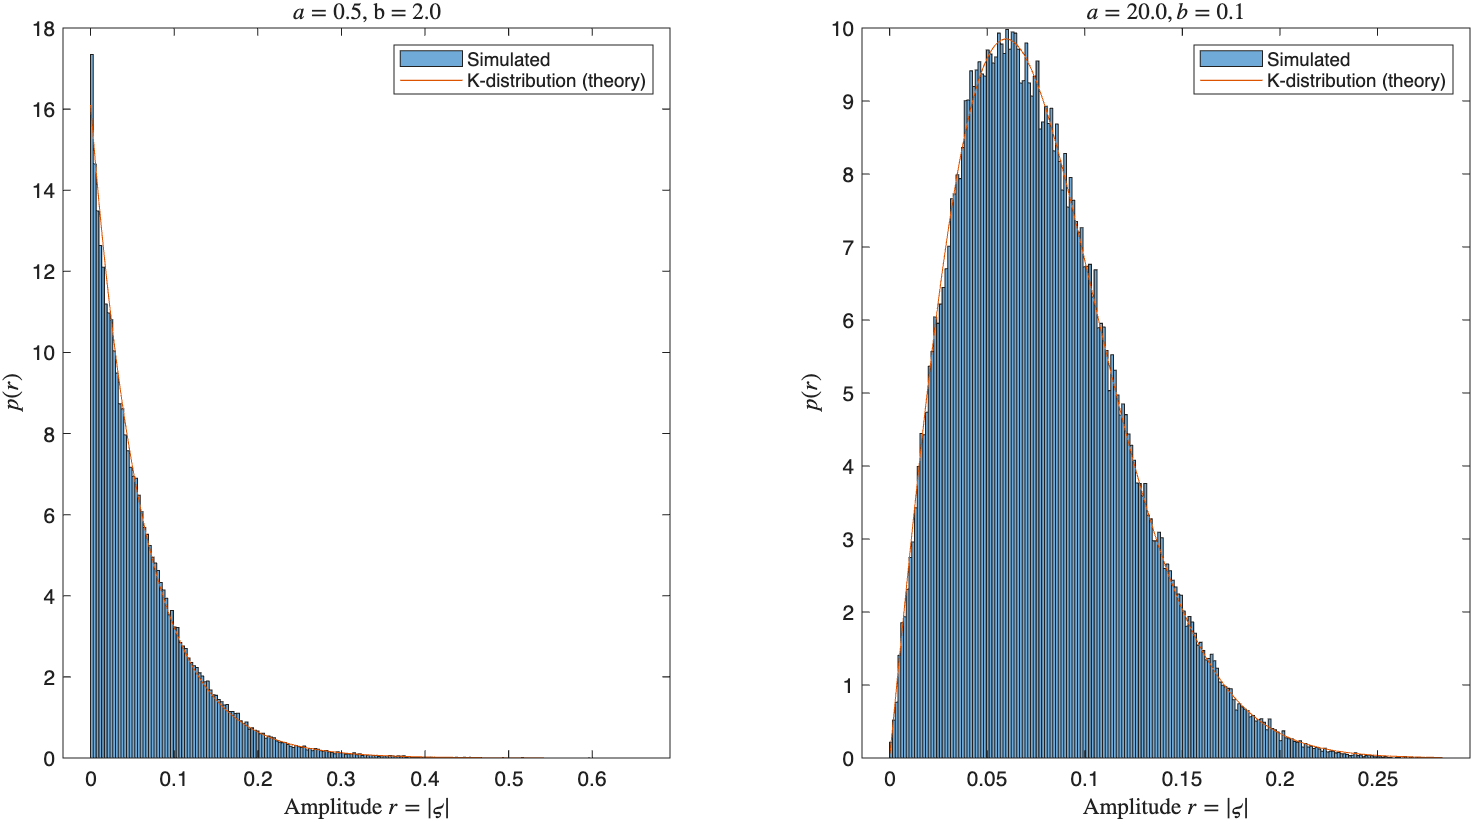
\includegraphics[height=3.2cm,width=0.95\textwidth]{figs/kdist_clutter.png}
            {\scriptsize Simulated amplitude vs theory}
        \end{column}
        \begin{column}{0.4\textwidth}
            \centering
            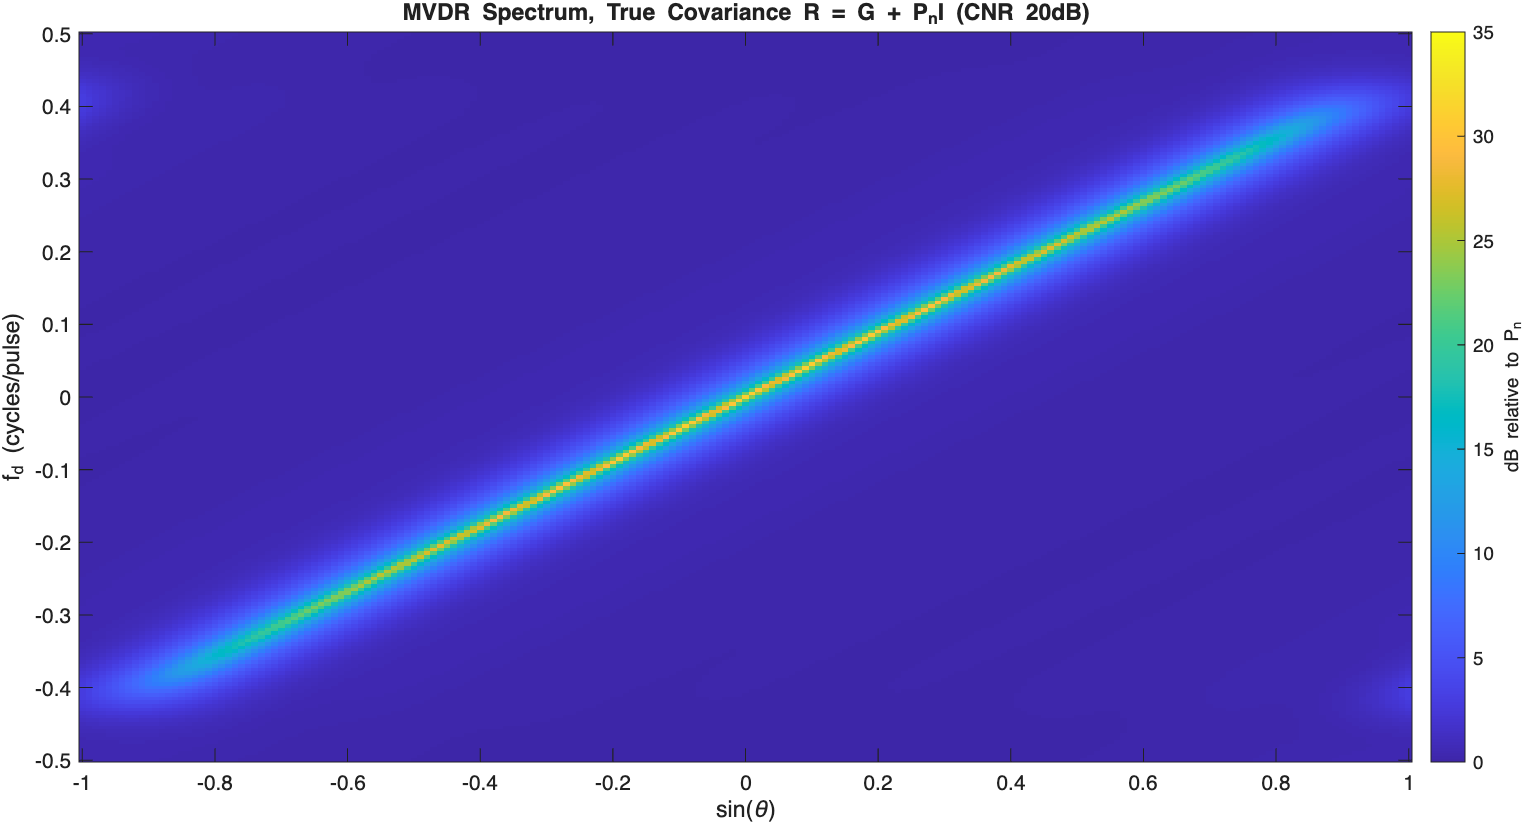
\includegraphics[height=3.2cm,width=0.92\textwidth]{true_MVDR.png}
            {\scriptsize Clutter ridge along $f_d = \beta f_s$}
        \end{column}
    \end{columns}
    \vspace{4mm}
    \textbf{Clutter-patch model} \cite{Melvin2004}: each range cell's clutter is the sum of echoes from the ground at that range\\
    % \begin{itemize}
    %     \item Ring of ground split into $N_\theta$ \textbf{patches}, each with its own angle and Doppler
    %     \item The integral over the ring is approximated by a \textbf{Riemann sum} over the patches
    %     \item K-distributed: scale each range cell by its own $\sqrt{\tau_k}$
    % \end{itemize}
    \vspace{4mm}
    {\color{structure}\textbf{Next:}} Use clutter generator for Monte Carlo comparison of $P_{fa}$ and $P_d$ for OKD vs AMF and NAMF
\end{frame}

%% 5.2 Sample vs True Covariance
\subsection{Sample vs True Covariance}
\begin{frame}{Sample vs True Covariance}
    \small
    \begin{columns}[c]
        \begin{column}{0.55\textwidth}
            \centering
            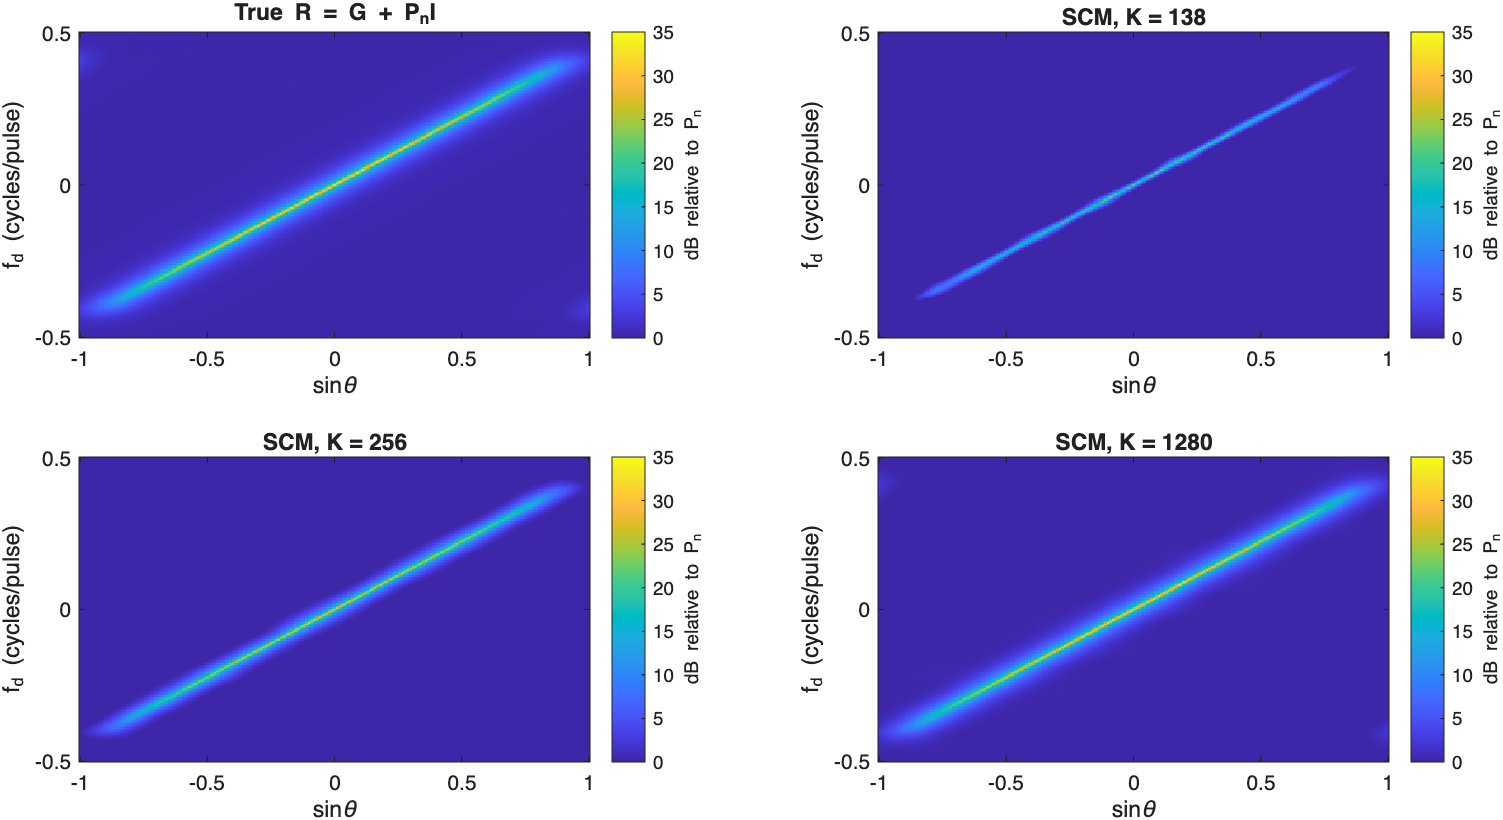
\includegraphics[height=3.7cm, keepaspectratio]{scm_vs_true.png}\\[2pt]
            {\scriptsize MVDR spectra: true $\mathbf{R}$ and SCM, $K = NM+10,\ 2NM,\ 10NM$}
        \end{column}
        \begin{column}{0.43\textwidth}
            What changes when $\hat{\mathbf{R}}$ replaces $\mathbf{R}$?
            \begin{itemize}
                \item Angle-Doppler MVDR spectra which shows where the interference is: ridge = clutter, floor = noise, for true and SCMs with different sample support, $K$
                \item Larger $K$: closer to the true $\mathbf{R}$
                \item Loss in smaller sample support.
                \item But this is the loss in a \textbf{linear} filter. What does the SCM cost inside the OKD?
            \end{itemize}
            \vspace{15mm}
        \end{column}
    \end{columns}
    \vspace{1mm}
    {\color{structure}\textbf{Next:}} OKD with $\hat{\mathbf{R}}$, texture removed or not; still CFAR? (sub-goal 2)
\end{frame}

%% 5.3 Projected Timeline
\begin{frame}{Projected Timeline}
    \raggedright\small\textbf{Gantt Chart}\par\vspace{1mm}
    \centering
    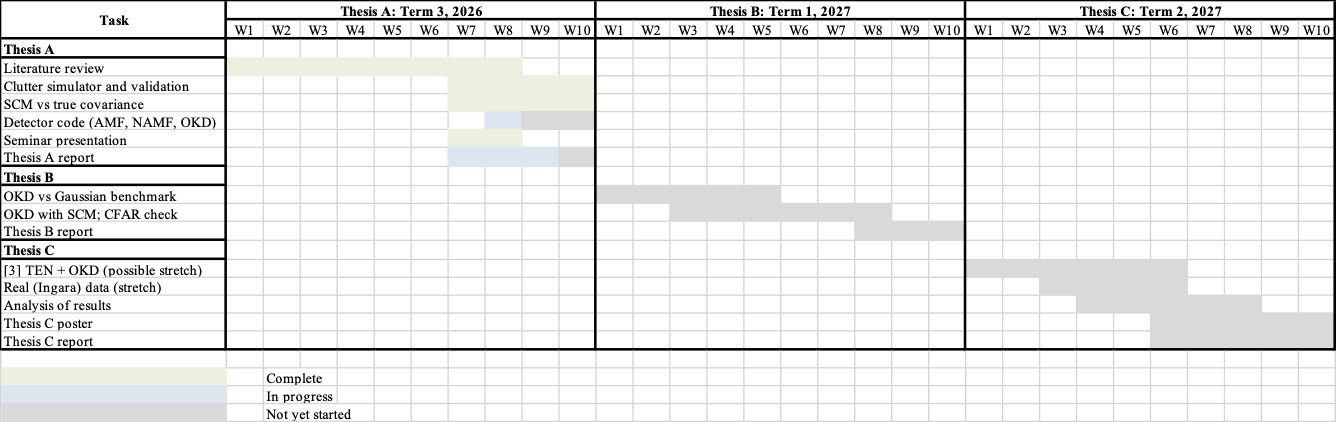
\includegraphics[width=0.88\textwidth]{gantt_chart.png}
    \par\vspace{1mm}
    \raggedright\footnotesize
    \begin{itemize}\setlength{\itemsep}{1pt}
        \item The approach is open-ended: tasks/goals are \textbf{open to change} and will be reviewed as simulations give more insight
        \item \textbf{Skills:}
        \begin{itemize}\footnotesize\setlength{\itemsep}{0pt}
            \item Statistical theory (estimation, detection)
            \item STAP signal processing
            \item Monte Carlo simulation in MATLAB
        \end{itemize}
    \end{itemize}
\end{frame}

%% ----- Summary ----- %%
\providecommand{\rc}[1]{\parbox[t]{0.68\textwidth}{\raggedright #1}}
\begin{frame}{Summary}
    \small
    \renewcommand{\arraystretch}{1.5}
    \begin{tabular}{@{}l l@{}}
        \toprule
        \textbf{Problem} & \rc{Small targets at sea are hidden in spiky, heterogeneous K-distributed clutter} \\
        \textbf{Now} & \rc{Gaussian detectors (AMF, NAMF, GLRT) and practical heterogeneous detectors (SDS, hybrid, TEN): degraded detection performance and loss of CFAR} \\
        \textbf{Gap} & \rc{The OKD is optimal for K clutter but clairvoyant: it needs the true $\mathbf{G}$ and texture $\tau$ statistics} \\
        \textbf{Aim} & \rc{To investigate a practical implementation of the OKD} \\
        \textbf{Preliminary} & \rc{Validated K-clutter simulator; detectors coded; effect of the SCM vs the true covariance} \\
        \textbf{Next} & \rc{OKD vs Gaussian $P_d$ curves; OKD with the SCM and its CFAR behaviour} \\
        \bottomrule
    \end{tabular}
    \vspace{5mm}
    \begin{center}
        {\Large \textbf{Thank you. Questions?}}
    \end{center}
\end{frame}

\appendix
%% ----- References ------ %%
{
\setbeamertemplate{headline}{}
\begin{frame}[allowframebreaks]{References}
    \printbibliography[heading=none]
\end{frame}
}

% %% ----- Backup Slides ----- %%
% %% ----- B1: Estimating the shape parameter ------ %%
% \begin{frame}{Backup: Estimating the Shape Parameter $a$}
%     \small
%     From clutter-only gates, use the intensity $z = |x|^2$ of each sample
%     \begin{columns}[T]
%         \begin{column}{0.5\textwidth}
%             \textbf{Method of moments}
%             \[ m = \frac{\langle z^2\rangle}{\langle z\rangle^2} = 2\Big(1+\frac{1}{a}\Big)
%                \;\Rightarrow\; \hat a = \frac{2}{m-2} \]
%             Gaussian clutter: $m = 2$, so $\hat a \to \infty$
%             \vspace{1mm}

%             \textbf{Better estimators}
%             \begin{itemize}
%                 \item $\langle z\log z\rangle$ estimator: lower variance
%                 \item Maximum likelihood: best, but numerical
%             \end{itemize}
%         \end{column}
%         \begin{column}{0.47\textwidth}
%             \textbf{Catches}
%             \begin{itemize}
%                 \item Noise makes clutter look more Gaussian: $\hat a$ biased \textbf{up}
%                 \item Samples in one gate share $\tau$: independent samples $\approx$ number of \textbf{gates}, not $NM\times$ gates
%                 \item $a$ itself varies across the scene
%             \end{itemize}
%             \vspace{1mm}
%             \textbf{Typical values}: $a<1$ very spiky, $a\gtrsim 20$ close to Gaussian
%         \end{column}
%     \end{columns}
%     \vspace{1mm}
%     \begin{block}{Sub-goal 3}
%         How much does the OKD lose when it uses $\hat a$ instead of the true $a$?
%     \end{block}
% \end{frame}

% %% ----- B2: Covariance estimators for K clutter ------ %%
% \begin{frame}{Backup: An ML Covariance Estimate for K Clutter?}
%     \small
%     \begin{columns}[T]
%         \begin{column}{0.5\textwidth}
%             \textbf{$\tau_k$ as unknown constants}: ML gives the \textbf{fixed-point (Tyler)} estimator \cite{Gini2002}:
%             \[ \hat{\mathbf{G}} = \frac{L}{K}\sum_{k=1}^{K}\frac{\mathbf{z}_k\mathbf{z}_k^H}{\mathbf{z}_k^H\hat{\mathbf{G}}^{-1}\mathbf{z}_k} \]
%             \begin{itemize}
%                 \item Each gate divided by its own power: $\tau_k$ cancels
%                 \item Same answer whatever the texture pdf
%                 \item Iterate from $\hat{\mathbf{G}}_0 = \mathbf{I}$; one step = NSCM
%             \end{itemize}
%         \end{column}
%         \begin{column}{0.47\textwidth}
%             \textbf{Treat $\tau_k$ as random (gamma)}
%             \begin{itemize}
%                 \item Likelihood needs $\int$ over every $\tau_k$: no closed-form ML
%                 \item Needs $a$ as well
%             \end{itemize}
%             \vspace{1mm}
%             \textbf{Why the thesis starts with the SCM}
%             \begin{itemize}
%                 \item It is what current detectors use
%                 \item Thermal noise breaks the FP's scale invariance ($\tau_k\mathbf{G} + \sigma^2\mathbf{I}$)
%                 \item FP is a natural next step after sub-goal 2
%             \end{itemize}
%         \end{column}
%     \end{columns}
%     \vspace{1mm}
%     \textbf{Scale:} only $\tau\mathbf{G}$ is identifiable, so fix $\mathbb{E}[\tau] = 1$ or $\mathrm{tr}(\mathbf{G}) = L$
% \end{frame}

% %% ----- B3: NAMF, Kelly and the RMB rule ------ %%
% \providecommand{\bnote}[1]{\parbox[c]{0.3\textwidth}{\raggedright\footnotesize #1}}
% \begin{frame}{Backup: NAMF, Kelly's GLRT and the RMB Rule}
%     \small
%     \begin{center}
%     \begin{tabular}{@{}l c l@{}}
%         \toprule
%         AMF & $\dfrac{|\mathbf{s}^H\hat{\mathbf{R}}^{-1}\mathbf{x}|^2}{\mathbf{s}^H\hat{\mathbf{R}}^{-1}\mathbf{s}}$ & \bnote{Two-step GLRT: SCM plugged into the matched filter} \\ \addlinespace[3mm]
%         NAMF & $\dfrac{|\mathbf{s}^H\hat{\mathbf{R}}^{-1}\mathbf{x}|^2}{(\mathbf{s}^H\hat{\mathbf{R}}^{-1}\mathbf{s})(\mathbf{x}^H\hat{\mathbf{R}}^{-1}\mathbf{x})}$ & \bnote{Scale-invariant in $\mathbf{x}$: CFAR to the CUT's own power} \\ \addlinespace[3mm]
%         Kelly & $\dfrac{|\mathbf{s}^H\hat{\mathbf{R}}^{-1}\mathbf{x}|^2}{(\mathbf{s}^H\hat{\mathbf{R}}^{-1}\mathbf{s})(K + \mathbf{x}^H\hat{\mathbf{R}}^{-1}\mathbf{x})}$ & \bnote{One-step GLRT: CUT and training together} \\
%         \bottomrule
%     \end{tabular}
%     \end{center}
%     \vspace{1mm}
%     \begin{block}{How much training data? \cite{Reed1974}}
%         SINR loss of the SCM filter $\rho \sim \mathrm{Beta}(K-L+2,\,L-1)$, so $\mathbb{E}[\rho] = \frac{K-L+2}{K+1}$.
%         Average loss of 3 dB needs $K \approx 2L$. With $N=8$, $M=16$: $L = 128$, so about 256 alike gates.
%     \end{block}
% \end{frame}

% %% ----- B4: OKD in detail ------ %%
% \begin{frame}{Backup: The OKD in Detail \cite{Gini1998}}
%     \small
%     \textbf{Quadratic forms} (unknown $\alpha$ replaced by its ML estimate, GLRT):
%     \[ q_0 = \mathbf{x}^H\mathbf{G}^{-1}\mathbf{x}, \qquad
%        q_1 = q_0 - \frac{|\mathbf{s}^H\mathbf{G}^{-1}\mathbf{x}|^2}{\mathbf{s}^H\mathbf{G}^{-1}\mathbf{s}} \]
%     $q_1$ = whitened power left once the best target along $\mathbf{s}$ is removed.
%     \vspace{1mm}

%     \textbf{Gamma texture, no noise}: $f_\tau(\tau) = \frac{a^a}{\Gamma(a)}\tau^{a-1}e^{-a\tau}$ gives
%     \[ h(q) = \int_0^\infty \tau^{-L} e^{-q/\tau} f_\tau(\tau)\,d\tau
%        \;\propto\; q^{\frac{a-L}{2}}\, K_{L-a}\big(2\sqrt{a q}\big) \]
%     \vspace{-2mm}
%     \begin{itemize}
%         \item $K_\nu$: modified Bessel function, hence ``K-distribution''
%         \item With noise, $\mathbf{R} = \tau\mathbf{G} + \sigma^2\mathbf{I}$ has no closed form: rotate to $\mathbf{G}$'s eigenbasis and integrate over $\tau$ numerically
%         \item Random (Swerling I) amplitude instead of GLRT: extra term in the $q_1$ denominator; same at high SCR
%     \end{itemize}
% \end{frame}

% %% ----- B5: TEN in detail ------ %%
% \begin{frame}{Backup: Texture Estimation and Normalisation (TEN) \cite{Aboutanios2020}}
%     \small
%     \begin{enumerate}
%         \item SDS estimate from sub-windows of each gate: $\hat{\mathbf{Q}}$ (CUT) and $\hat{\mathbf{R}}_k$ (gate $k$)
%         \item Texture ratio of gate $k$ to the CUT:
%         \[ \zeta_k = \tfrac{1}{L}\,\mathrm{tr}\big(\hat{\mathbf{Q}}^{-1}\hat{\mathbf{R}}_k\big) \approx \tau_k/\tau_T \]
%         \item Rescale to the CUT's power, $\tilde{\mathbf{R}}_k = \hat{\mathbf{R}}_k/\zeta_k \approx \tau_T\mathbf{G}$, and pool:
%         \[ \hat{\boldsymbol{\Sigma}}_\text{TEN} = \frac{(K-1)\hat{\mathbf{Q}} + \sum_k \tilde{\mathbf{R}}_k}{2K-1} \]
%         \item Use $\hat{\boldsymbol{\Sigma}}_\text{TEN}$ in an AMF-type statistic
%     \end{enumerate}
%     \vspace{1mm}
%     \begin{block}{What TEN gives, and what it does not}
%         Texture \textbf{ratios} and $\tau_T\mathbf{G}$; never $\tau$ and $\mathbf{G}$ separately. Feeding these into the OKD is the stretch goal.
%     \end{block}
% \end{frame}

% %% ----- B6: SCM details ------ %%
% \begin{frame}{Backup: Why the SCM, and Why Leave Out the CUT?}
%     \small
%     \begin{columns}[T]
%         \begin{column}{0.5\textwidth}
%             \textbf{SCM is ML for i.i.d.\ Gaussian training}
%             \[ \log p = -K\big(\log|\mathbf{R}| + \mathrm{tr}(\mathbf{R}^{-1}\hat{\mathbf{R}})\big) + \text{const} \]
%             maximised at $\mathbf{R} = \hat{\mathbf{R}} = \frac{1}{K}\sum_k\mathbf{z}_k\mathbf{z}_k^H$
%             \vspace{1mm}
%             \begin{itemize}
%                 \item Unbiased: $\mathbb{E}[\hat{\mathbf{R}}] = \mathbf{R}$
%                 \item But $\mathbb{E}[\hat{\mathbf{R}}^{-1}] = \tfrac{K}{K-L}\mathbf{R}^{-1}$ (inverse Wishart)
%                 \item Needs $K \ge L$ to be invertible
%             \end{itemize}
%         \end{column}
%         \begin{column}{0.47\textwidth}
%             \textbf{Why not use the CUT?}
%             \begin{itemize}
%                 \item A target in the training is treated as interference and \textbf{nulled}: self-cancellation
%                 \item \textbf{Guard cells} stop target energy that spreads into neighbouring gates
%             \end{itemize}
%             \vspace{1mm}
%             \textbf{In K clutter}
%             \begin{itemize}
%                 \item $\mathbb{E}[\hat{\mathbf{R}}] = \bar\tau\mathbf{G} + \sigma^2\mathbf{I}$: the \emph{average} power, not the CUT's $\tau_T$
%                 \item One spiky gate can dominate the sum
%             \end{itemize}
%         \end{column}
%     \end{columns}
% \end{frame}

% %% ----- B7: MVDR and the floor drop ------ %%
% \begin{frame}{Backup: MVDR Spectrum and the $(K-L)/K$ Floor}
%     \small
%     \begin{columns}[T]
%         \begin{column}{0.5\textwidth}
%             \textbf{MVDR (Capon) spectrum}
%             \[ P(f_s,f_d) = \frac{1}{\mathbf{s}^H\mathbf{R}^{-1}\mathbf{s}} \]
%             \begin{itemize}
%                 \item Minimum output power with unit gain on $\mathbf{s}$
%                 \item Much sharper than the Fourier spectrum $\mathbf{s}^H\mathbf{R}\mathbf{s}$: shows the thin ridge
%             \end{itemize}
%         \end{column}
%         \begin{column}{0.47\textwidth}
%             \textbf{With the SCM}
%             \[ \mathbb{E}\big[\mathbf{s}^H\hat{\mathbf{R}}^{-1}\mathbf{s}\big] = \frac{K}{K-L}\,\mathbf{s}^H\mathbf{R}^{-1}\mathbf{s} \]
%             so the spectrum drops by about $\frac{K-L}{K}$
%             \vspace{1mm}
%             \begin{center}
%             \footnotesize
%             \begin{tabular}{lr}
%                 \toprule
%                 $K$ ($L = 128$) & $10\log_{10}\frac{K-L}{K}$ \\
%                 \midrule
%                 $L+10$ & $-11.4$ dB \\
%                 $2L$ & $-3.0$ dB \\
%                 $10L$ & $-0.5$ dB \\
%                 \bottomrule
%             \end{tabular}
%             \end{center}
%         \end{column}
%     \end{columns}
% \end{frame}

\end{document}	